\subsection{COASSOCIATIVITY, COCOMMUTATIVITY, COUNIT}

Let E be a cogebra, c its coproduct, N, N', N'' three A-modules and m a bilinear mapping of N × N' into N''. Let \(\tilde{m}:N \otimes_{A} N' \to N''\) denote the A-linear mapping corresponding to m. If \(u:E \to N\) , \(v:E \to N'\) are two A-linear mappings, we derive an A-linear mapping \(u \otimes v:E \otimes_{A} E \to N \otimes_{A} N'\) and a composite A-linear mapping of E into N'':

\[
m (u, v): \mathrm{E} \xrightarrow {c} \mathrm{E} \otimes_ {\mathrm{A}} \mathrm{E} \xrightarrow {u \otimes v} \mathrm{N} \otimes_ {\mathrm{A}} \mathrm{N} ^ {\prime} \xrightarrow {\tilde {m}} \mathrm{N} ^ {\prime \prime}.\tag{11}
\]

Clearly we have thus defined an A-bilinear mapping \((u, v) \mapsto m(u, v)\) of \(\operatorname{Hom}_{\mathbf{A}}(\mathbf{E}, \mathbf{N}) \times \operatorname{Hom}_{\mathbf{A}}(\mathbf{E}, \mathbf{N}')\) into \(\operatorname{Hom}_{\mathbf{A}}(\mathbf{E}, \mathbf{N}'')\) .

When E is a graded cogebra, N, N', N'' graded A-modules of the same type and \(\tilde{m}\) a graded homomorphism of degree k of N \(\otimes_{A}N'\) into N'', then, if u (resp. v) is a graded homomorphism of degree p (resp. q), \(m(u,v)\) is a graded homomorphism of degree \(p + q + k\) .

Examples. (1) Take E to be the graded cogebra T(M) (no. 1) and suppose that N, N', N'' have the trivial graduation. A graded homomorphism of degree -p of T(M) into N (resp. N', N'') then corresponds to a multilinear mapping of M\^{}p into N (resp. N', N''). Given a multilinear mapping u: M\^{}p → N and a multilinear mapping v: M\^{}q → N', the above method allows us to deduce a multilinear mapping m(u, v): M\^{}\{p+q\} → N'' called the product (relative to m) of u and v. Formulae (3) (no. 1) and (11) show that, for x\_1, . . ., x\_p+q in M,

\[
(m (u, v)) \left(x _ {1}, \dots , x _ {p + q}\right) = m \left(u \left(x _ {1}, \dots , x _ {p}\right), v \left(x _ {p + 1}, \dots , x _ {p + q}\right)\right).
\]

\begin{enumerate}
\def\labelenumi{(\arabic{enumi})}
\setcounter{enumi}{1}
\tightlist
\item
  Take E to be the graded cogebra S(M) (no. 1), preserving the same hypotheses on N, N', N''. A graded homomorphism of degree -p of S(M) into N then corresponds to a symmetric multilinear mapping of M \(^{p}\) into N (§ 6, no. 3). Then we derive from a symmetric multilinear mapping u: M \(^{p}\) → N and a symmetric multilinear mapping v: M \(^{q}\) → N' a symmetric multilinear mapping m(u, v): M \(^{p+q}\) → N'', also denoted (to avoid confusion) by \(u \cdot_{m} v\) (or even \(u \cdot v\)) and called the symmetric product (relative to m) of u and v. Formulae (6) (no. 1) and (11) show that, for x₁, \ldots, x \(_{p+q}\) in M,
\end{enumerate}

\[
(u \cdot_{m} v) (x _ {1}, \dots , x _ {p + q}) = \sum_ {\sigma} m (u (x _ {\sigma (1)}, \dots , x _ {\sigma (p)}), v (x _ {\sigma (p + 1)}, \dots , x _ {\sigma (p + q)}))
\]

the summation being taken over permutations \(\sigma\in\mathfrak{S}_{p+q}\) which are increasing on each of the intervals \([1,p]\) and \([p+1,p+q]\) .

\begin{enumerate}
\def\labelenumi{(\arabic{enumi})}
\setcounter{enumi}{2}
\tightlist
\item
  Take E to be the graded cogebra \(\bigwedge (\mathbf{M})\) (no. 1). Then we deduce similarly from an alternating multilinear mapping \(u: \mathbf{M}^p \to \mathbf{N}\) and an alternating multilinear mapping \(v: \mathbf{M}^q \to \mathbf{N}'\) an alternating multilinear mapping \(m(u, v): \mathbf{M}^{p + q} \to \mathbf{N}''\) , also denoted by \(u \wedge_m v\) or \(u \wedge v\) and called the alternating product (relative to \(m\) ) of \(u\) and \(v\) . Formulae (9) (no. 1) and (11) show in this case that, for \(x_1, \ldots, x_{p + q}\) in \(\mathbf{M}\) ,
\end{enumerate}

\[
(u \wedge_ {m} v) (x _ {1}, \dots , x _ {p + q}) = \sum_ {\sigma} \varepsilon_ {\sigma} m (u (x _ {\sigma (1)}, \dots , x _ {\sigma (p)}), v (x _ {\sigma (p + 1)}, \dots , x _ {\sigma (p + q)}))
\]

the summation again being taken over permutations \(\sigma \in \mathfrak{S}_{p + q}\) which are increasing on each of the intervals \([1, p]\) and \([p + 1, p + q]\) .

We return to the case where E is an arbitrary graded cogebra (of type N) and assume that the three modules N, N', N'' are all equal to the underlying A-module of a graded A-algebra B of type Z, the mapping m being multiplication in B, so that \(\tilde{m}:B\otimes_{A}B\to B\) is a graded A-linear mapping of degree 0. Thus a graded A-algebra structure is obtained on the graded A-module \(\operatorname{Homgr}_{A}(E,B)=C\) .

In particular, suppose that B = A (with the trivial graduation), so that \(\operatorname{Homgr}_{\mathbf{A}}(\mathbf{E}, \mathbf{A})\) is the graded dual \(E^{*gr}\) , which thus has a graded A-algebra structure.

Let F be another graded cogebra \(c'\) its coproduct and \(\phi:E\to F\) a graded cogebra morphism (no. 1); then the canonical graded morphism

\[
\tilde {\phi} = \operatorname{Hom} (\phi , 1 _ {B}): \operatorname{Homgr} _ {A} (F, B) \rightarrow \operatorname{Homgr} _ {A} (E, B)
\]

is a graded algebra homomorphism. For \(u, v\) in \(\operatorname{Homgr}_{\mathbf{A}}(\mathbf{F}, \mathbf{B})\) and \(x \in \mathbf{E}\) ,

\[
(\tilde {\phi} (u v)) (x) = (u v) (\phi (x)) = m ((u \otimes v) (c ^ {\prime} (\phi (x))))
\]

But by hypothesis \(c'(\phi(x)) = (\phi \otimes \phi)(c(x))\) , hence

\[
(u \otimes v) (c ^ {\prime} (\phi (x))) = (\tilde {\phi} (u) \otimes \tilde {\phi} (v)) (c (x))
\]

and therefore \(\tilde{\phi}(uv) = \tilde{\phi}(u)\tilde{\phi}(v)\) , which proves our assertion.

In particular, the graded transpose \({}^{t}\phi: \mathrm{F}^{*gr} \to \mathrm{E}^{*gr}\) is a graded algebra homomorphism.

Remark. Suppose that the \(E_{p}\) are finitely generated projective A-modules, so that the graded A-modules ( \(E \otimes_{A} E)^{*gr}\) and \(E^{*gr} \otimes_{A} E^{*gr}\) can be canonically identified (II, §4, no. 4, Corollary 1 to Proposition 4). If also the A-modules \(A \otimes_{A} A\) and A are then canonically identified (II, §3, no. 4), the linear mapping \(E^{*gr} \otimes_{A} E^{*gr} \to E^{*gr}\) which defines multiplication in \(E^{*gr}\) can be called the graded transpose of the coproduct c.

PROPOSITION 1. Let E be a cogebra over A. In order that, for every associative A-algebra B, the A-algebra \(\operatorname{Hom}_{\mathbf{A}}(\mathbf{E}, \mathbf{B})\) be associative, it is necessary and sufficient that the coproduct \(c: \mathbf{E} \to \mathbf{E} \otimes_{\mathbf{A}} \mathbf{E}\) be such that the diagram

\begin{enumerate}
\def\labelenumi{(\arabic{enumi})}
\setcounter{enumi}{11}
\tightlist
\item
\end{enumerate}

\pandocbounded{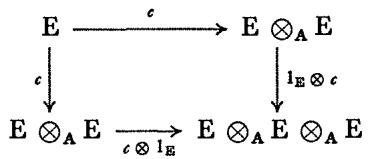
\includegraphics[keepaspectratio]{images/part004_a79ed2ff.jpg}}

be commutative.

Let B be an associative A-algebra and u, v, w three elements of \(\mathbf{C} = \operatorname{Hom}_{\mathbf{A}}(\mathbf{E}, \mathbf{B})\) . Let \(m_{3}\) denote the A-linear mapping \(B \otimes_{A} B \otimes_{A} B \to B\) which maps \(b \otimes b' \otimes b''\) to \(bb'b''\) . By definition of the product on the algebra C, \((uv)w\) is the composite mapping

\[
\mathrm{E} \xrightarrow {c} \mathrm{E} \otimes \mathrm{E} \xrightarrow {c \otimes 1 _ {\mathrm{E}}} \mathrm{E} \otimes \mathrm{E} \otimes \mathrm{E} \xrightarrow {u \otimes v \otimes w} \mathrm{B} \otimes \mathrm{B} \otimes \mathrm{B} \xrightarrow {m _ {3}} \mathrm{B}
\]

whilst \(u(vw)\) is the composite mapping

\[
\mathrm{E} \xrightarrow {c} \mathrm{E} \otimes \mathrm{E} \xrightarrow {1 _ {\mathrm{E}} \otimes c} \mathrm{E} \otimes \mathrm{E} \otimes \mathrm{E} \xrightarrow {u \otimes v \otimes w} \mathrm{B} \otimes \mathrm{B} \otimes \mathrm{B} \xrightarrow {m _ {3}} \mathrm{B}.
\]

It follows that if diagram (12) is commutative, the algebra \(\operatorname{Hom}_{\mathbf{A}}(\mathbf{E}, \mathbf{B})\) is associative for every associative A-algebra B. To establish the converse, it suffices to show that there exists an associative A-algebra B and three A-linear mappings \(u, v, w\) of E into B such that the mapping \(m_3 \circ (u \otimes v \otimes w)\) of \(\mathbf{E} \otimes \mathbf{E} \otimes \mathbf{E}\) into B is injective. Take B to be the A-algebra \(\mathsf{T}(\mathbf{E})\) and \(u, v, w\) the canonical mapping of E into \(\mathsf{T}(\mathbf{E})\) . The mapping \(m_3 \circ (u \otimes v \otimes w)\) is then the canonical mapping \(\mathbf{E} \otimes \mathbf{E} \otimes \mathbf{E} = \mathsf{T}^3(\mathbf{E}) \to \mathsf{T}(\mathbf{E})\) , which is injective.

When the cogebra E satisfies the condition of Proposition 1, it is said to be coassociative.

Examples. (4) It is immediately verified that the cogebra A (no. 1, Example (1)) the cogebra \(\mathbf{A}^{(\mathbf{X})}\) (no. 1, Example 4) and the cogebra \(\mathbf{T}(\mathbf{M})\) (no. 1, Example 5) are coassociative. If B is an associative A-algebra which is a finitely generated projective A-module, the cogebra \(\mathbf{B}^*\) (no. 1, Example 3) is coassociative: for the commutativity of diagram (12) then follows by transposition from that of the diagram which expresses the associativity of B ( \(\S\) 1, no. 3). Conversely, the same argument and the canonical identification of the A-module B with its bidual (II, § 2, no. 7, Corollary 4 to Proposition 13) show that if the cogebra \(\mathbf{B}^*\) is coassociative, the algebra \(\mathbf{B}\) is associative. Finally, the cogebras \(\mathsf{S}(\mathbf{M})\) and \(\bigwedge (\mathbf{M})\) (no. 1, Examples 6 and 7) are coassociative; this follows from the commutativity of the diagram

\[
\begin{array}{c} \mathrm{M} \xrightarrow {\Delta} \mathrm{M} \times \mathrm{M} \\ \Delta \Biggl \downarrow \\ \mathrm{M} \times \mathrm{M} \xrightarrow [ \Delta \times 1 _ {\mathrm{M}} ]{} \mathrm{M} \times \mathrm{M} \times \mathrm{M} \end{array}
\]

the functorial properties of \(\mathsf{S}(\mathbf{M})\) ( \(\S 6\) , no. 2) and \(\bigwedge (\mathbf{M})\) ( \(\S 7\) , no. 2), which give the corresponding commutative diagrams

\[
\left\{ \begin{array}{c} \mathsf {S} (\mathbf {M}) \xrightarrow {\mathsf {S} (\Delta)} \mathsf {S} (\mathbf {M} \times \mathbf {M}) \\ \mathsf {S} (\Delta) \Biggl \downarrow \qquad \qquad \qquad \qquad \qquad \qquad \qquad \qquad \qquad \qquad \qquad \qquad \qquad \qquad \qquad \qquad \qquad \qquad \qquad \qquad \qquad \qquad \qquad \qquad \qquad \qquad \qquad \qquad \qquad \qquad \qquad \qquad \qquad \qquad \mathsf {S} (1 _ {\mathbf {M}} \times \Delta) \\ \mathsf {S} (\mathbf {M} \times \mathbf {M}) \xrightarrow [ \mathsf {S} (\Delta \times 1 _ {\mathbf {M}}) ]{\mathsf {S} (\Delta \times 1 _ {\mathbf {M}})} \mathsf {S} (\mathbf {M} \times \mathbf {M} \times \mathbf {M}) \\ \bigwedge (\mathbf {M}) \xrightarrow {\bigwedge (\Delta)} \bigwedge (\mathbf {M} \times \mathbf {M}) \\ \bigwedge (\Delta) \Biggl \downarrow \qquad \qquad \qquad \qquad \qquad \qquad \qquad \qquad \qquad \qquad \qquad \qquad \qquad \bigwedge (1 _ {\mathbf {M}} \times \Delta) \\ \bigwedge (\mathbf {M} \times \mathbf {M}) \xrightarrow [ \bigwedge (\Delta \times 1 _ {\mathbf {M}}) ]{\bigwedge (\Delta \times 1 _ {\mathbf {M}})} \bigwedge (\mathbf {M} \times \mathbf {M} \times \mathbf {M}) \end{array} \right.\tag{14}
\]

and the existence and functoriality of canonical isomorphisms for symmetric and exterior algebras of a direct sum (§ 6, no. 6 and § 7, no. 7).

PROPOSITION 2. Let E be a cogebra over A. In order that, for every commutative A-algebra B, the A-algebra \(\operatorname{Hom}_{\mathbf{A}}(\mathbf{E}, \mathbf{B})\) be commutative, it is necessary and sufficient that the coproduct \(c: \mathbf{E} \to \mathbf{E} \otimes_{\mathbf{A}} \mathbf{E}\) be such that the diagram

\begin{enumerate}
\def\labelenumi{(\arabic{enumi})}
\setcounter{enumi}{14}
\tightlist
\item
\end{enumerate}

\pandocbounded{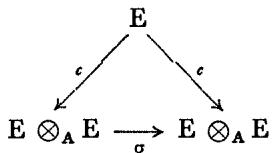
\includegraphics[keepaspectratio]{images/part004_07c99209.jpg}}

(where \(\sigma\) is the symmetry homomorphism such that \(\sigma(x \otimes y) = y \otimes x\) ) is commutative (in other words, it suffices that the cogebra E be identical with its opposite (no. 1, Example 2).

Let B be a commutative A-algebra and u, v two elements of C = Hom\_A(E, B).

By definition of the product in C, uv and vu are respectively equal to the composite mappings

\[
\mathrm{E} \xrightarrow {c} \mathrm{E} \otimes \mathrm{E} \xrightarrow {u \otimes v} \mathrm{B} \otimes \mathrm{B} \xrightarrow {m} \mathrm{B}
\]

and

\[
\mathrm{E} \xrightarrow {c} \mathrm{E} \otimes \mathrm{E} \xrightarrow {v \otimes u} \mathrm{B} \otimes \mathrm{B} \xrightarrow {m} \mathrm{B}.
\]

It follows that if diagram (15) is commutative the algebra \(\operatorname{Hom}_{\mathbf{A}}(\mathbf{E}, \mathbf{B})\) is commutative for every commutative A-algebra B. To establish the converse, it suffices to show that there exist a commutative A-algebra B and two A-linear mappings \(u, v\) of E into B such that \(m \circ (u \otimes v): \mathbf{E} \otimes \mathbf{E} \to \mathbf{B}\) is injective. Take B to be the algebra \(\mathsf{S}(\mathbf{E} \oplus \mathbf{E})\) and \(u\) (resp. \(v\) ) the composition of the canonical mapping \(\mathbf{E} \oplus \mathbf{E} \to \mathsf{S}(\mathbf{E} \oplus \mathbf{E})\) and the mapping \(x \mapsto (x, 0)\) (resp. \(x \mapsto (0, x)\) ) of E into \(\mathbf{E} \oplus \mathbf{E}\) . If \(h: \mathsf{S}(\mathbf{E}) \otimes \mathsf{S}(\mathbf{E}) \to \mathsf{S}(\mathbf{E} \otimes \mathbf{E})\) is the canonical isomorphism ( \(\S 6\) , no. 6, Proposition 9) and \(\lambda: \mathbf{E} \to \mathsf{S}(\mathbf{E})\) is the canonical mapping, then \(h^{-1} \circ m \circ (u \otimes v) = \lambda \otimes \lambda\) . Now \(\lambda \otimes \lambda\) is injective, for \(\lambda(\mathbf{E})\) is a direct factor of \(\mathsf{S}(\mathbf{E})\) (II, § 3, no. 7, Corollary 5 to Proposition 7).

When the cogebra E satisfies the condition of Proposition 2, it is said to be cocommutative.

Examples. (5) It is immediate that the cogebra A (no. 1, Example 1) and the cogebra \(\mathbf{A}^{(\mathbf{X})}\) (II, § 11, no. 1, Example 4) are cocommutative. It follows from formula (5) of no. 1 that the cogebra S(M) is cocommutative. Finally, for an A-algebra B such that the A-module B is projective and finitely generated to have the property that the cogebra \(\mathbf{B}^*\) (no. 1, Example 3) is cocommutative, it is necessary and sufficient that B be commutative; for (using the canonical identification of the A-module B with its bidual (II, § 2, no. 7)), this follows from the fact that the commutativity of diagram (14) is equivalent by transposition to that of the diagram which expressed the commutativity of B (§ 1, no. 3).

PROPOSITION 3. Let E be a cogebra over A. In order that, for every unital A-algebra B, the A-algebra \(\operatorname{Hom}_{\mathbf{A}}(\mathbf{E},\mathbf{B})\) be unital, it is necessary and sufficient that there exist a linear form \(\gamma\) on E rendering commutative the diagrams

\begin{enumerate}
\def\labelenumi{(\arabic{enumi})}
\setcounter{enumi}{15}
\tightlist
\item
\end{enumerate}

\pandocbounded{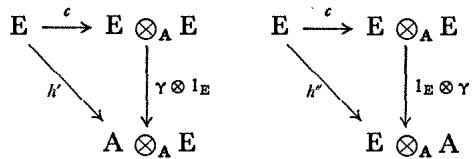
\includegraphics[keepaspectratio]{images/part004_cc0e83d1.jpg}}

where \(c: \mathbf{E} \to \mathbf{E} \otimes_{\mathbf{A}} \mathbf{E}\) is the coproduct and \(h'\) and \(h''\) the canonical isomorphisms (II, § 3, no. 4, Proposition 4). The unit of \(\operatorname{Hom}_{\mathbf{A}}(\mathbf{E}, \mathbf{B})\) is then the linear mapping \(x \mapsto \gamma(x)1\) (where 1 denotes the unit element of B).

Let \(\gamma\) be a linear form on E rendering diagram (16) commutative. Let B be a unital A-algebra with unit element 1, \(\eta: \mathbf{A} \to \mathbf{B}\) the canonical mapping and \(v = \eta \circ \gamma\) the element of the A-algebra \(\mathbf{C} = \operatorname{Hom}_{\mathbf{A}}(\mathbf{E}, \mathbf{B})\) . For every element \(u \in \mathbf{C}\) , \(uv\) is the composite mapping

\[
\mathrm{E} \xrightarrow {c} \mathrm{E} \otimes \mathrm{E} \xrightarrow {1 _ {\mathrm{E}} \otimes \gamma} \mathrm{E} \otimes \mathrm{A} \xrightarrow {u \otimes \eta} \mathrm{B} \otimes \mathrm{B} \xrightarrow {m} \mathrm{B}.\tag{17}
\]

Then \(uv = m \circ (u \otimes \eta) \circ h'' = u\) . It is similarly proved that \(vu = u\) and hence \(v\) is unit element of C. Conversely, let the A-module A ⊕ E be given a unital algebra structure such that \((a, x)(a', x') = (aa', ax' + a'x)\) for \(a, a'\) in A and \(x, x'\) in E. Let B denote the A-algebra thus defined and let C be the A-algebra Hom \(_A(E, B)\) . Suppose that C is unital and let \(e: x \mapsto (\gamma(x), \lambda(x))\) be its unit element (where \(\gamma(x) \in A\) and \(\lambda(x) \in E\) ). On the other hand let \(f\) be the element \(x \mapsto (0, x)\) of C. An immediate calculation shows that \(fe\) is the element

\[
x \mapsto (0, (h ^ {\prime \prime}) ^ {- 1} ((1 _ {E} \otimes \gamma) (c (x))))
\]

of C. The condition \(fe = f\) implies the commutativity of the second diagram of (16) and it is similarly seen that the condition \(ef = f\) implies the commutativity of the first diagram of (16).

A linear form \(\gamma\) on E rendering diagrams (16) commutative is called a counit of the cogebra E. A cogebra admits at most one counit: for it is the unit element of the algebra \(\operatorname{Hom}_{\mathbf{A}}(\mathbf{E}, \mathbf{A})\) . A cogebra with a counit is called counital.

Examples. (6) The identity mapping is the counit of the cogebra A; on the cogebra \(\mathbf{A}^{(\mathbf{X})}\) (no. 1, Example 4) the linear form \(\gamma\) such that \(\gamma(e_x) = 1\) for all \(x \in \mathbf{X}\) is the counit. On the cogebra \(\mathbf{T}(\mathbf{M})\) (resp. \(\mathbf{S}(\mathbf{M}), \bigwedge(\mathbf{M})\) ) the linear form \(\gamma\) such that \(\gamma(1) = 1\) and \(\gamma(z) = 0\) for \(z\) in the \(\mathbf{T}^n(\mathbf{M})\) (resp. \(\mathbf{S}^n(\mathbf{M}), \bigwedge^n(\mathbf{M})\) ) for \(n \geqslant 1\) is the counit. Finally, let B be an A-algebra which is a finitely generated projective A-module and has a unit element \(e\) ; then on the cogebra \(\mathbf{B}^*\) (no. 1, Example 3) the linear form \(\gamma: x^* \mapsto \langle e, x^* \rangle\) is the counit, for this form is just the transpose of the A-linear mapping \(\eta_e: \xi \mapsto \xi e\) of A into B and by transposition the commutativity of diagrams (16) follows from that of the diagrams which express (using \(\eta_e\) ) the fact that \(e\) is unit element of B ( \(\S 1\) , no. 3); the same argument moreover shows that conversely, if the cogebra \(\mathbf{B}^*\) admits a counit \(\gamma\) , the transpose of \(\gamma\) defines a unit element \(e = {}^t\gamma(1)\) of B.

PROPOSITION 4. Let E be a cogebra admitting a counit \(\gamma\) and suppose that there exists in E an element \(e\) such that \(\gamma(e) = 1\) ; then E is the direct sum of the sub-A-modules Ae and \(\mathrm{E}_{\gamma} = \mathrm{Ker}(\gamma)\) and

\[
c (e) \equiv e \otimes e (\mathrm{mod.} \mathrm{E} _ {\gamma} \otimes \mathrm{E} _ {\gamma})\tag{18}
\]

\[
\left\{c (x) \equiv x \otimes e + e \otimes x (\mathrm{mod.} \mathrm{E} _ {\gamma} \otimes \mathrm{E} _ {\gamma}) \quad \text { for all } x \in \mathrm{E} _ {\gamma}. \right.
\]

The first assertion is immediate, for \(\gamma(x - \gamma(x)e) = 0\) and the relation \(\gamma(\alpha e) = 0\) implies \(\alpha = 0\) . Let \(c(e) = \sum_{i} s_i \otimes t_i\) , so that

\[
e = \sum_ {i} \gamma (s _ {i}) t _ {i} = \sum_ {i} \gamma (t _ {i}) s _ {i}
\]

by (16) and \(1 = \gamma(e) = \sum_{i} \gamma(s_i) \gamma(t_i)\) . Therefore

\[
\begin{array}{r l} \sum_ {i} (s _ {i} - \gamma (s _ {i}) e) \otimes (t _ {i} - \gamma (t _ {i}) e) & = \sum_ {i} s _ {i} \otimes t _ {i} - \sum_ {i} e \otimes \gamma (s _ {i}) t _ {i} \\ & - \sum_ {i} \gamma (t _ {i}) s _ {i} \otimes e \\ & + \sum_ {i} \gamma (s _ {i}) e \otimes \gamma (t _ {i}) e \end{array}
\]

which, by the above relation, is just \(c(e) - e \otimes e\) ; this therefore proves the first relation of (18). On the other hand the decomposition of E \(\otimes\) E as a direct sum

\[
\mathbf {A} (e \otimes e) \oplus ((\mathbf {A} e) \otimes \mathbf {E} _ {\gamma}) \oplus (\mathbf {E} _ {\gamma} \otimes (\mathbf {A} e)) \oplus (\mathbf {E} _ {\gamma} \otimes \mathbf {E} _ {\gamma})
\]

allows us to write, for \(x \in \mathbf{E}_{\gamma}\) , \(c(x) = \lambda(e \otimes e) + (e \otimes y) + (z \otimes e) + u\) where \(u = \sum_{j} v_{j} \otimes w_{j}, y, z\) and the \(v_{j}\) and \(w_{j}\) belong to \(\mathbf{E}_{\gamma}\) . The definition of the counit \(\gamma\) then gives \(x = \lambda e + y = \lambda e + z\) and, as \(\gamma(x) = 0\) , necessarily \(\lambda = 0, x = y = z\) , whence the second relation of (18).

Remark. Let C be a counital coassociative A-coalgebra, B a unital associative A-algebra and M a left B-module. The A-bilinear mapping \((b, m) \mapsto bm\) of \(B \times M\) into M defines an A-bilinear mapping

\[
\operatorname{Hom} _ {\mathbf {A}} (\mathrm{C}, \mathrm{B}) \times \operatorname{Hom} _ {\mathbf {A}} (\mathrm{C}, \mathrm{M}) \rightarrow \operatorname{Hom} _ {\mathbf {A}} (\mathrm{C}, \mathrm{M})
\]

by the general procedure described at the beginning of this no. It is immediately verified that this mapping defines on \(\operatorname{Hom}_{\mathbf{A}}(\mathbf{C}, \mathbf{M})\) a left module structure over the ring \(\operatorname{Hom}_{\mathbf{A}}(\mathbf{C}, \mathbf{B})\) .

